\chapter{Cơ sở lý thuyết}
\label{chp:02}

\section{Kiến trúc tập lệnh RISC-V}
\label{sec:risc-v}

\subsection{Lịch sử hình thành}

RISC-V là một kiến trúc tập lệnh (Instruction Set Architecture - ISA) 
dựa trên nguyên lý RISC (Reduced Instruction Set Computer), 
được đưa ra vào năm 2010 tại Phòng thí nghiệm Tính toán song song 
của Đại học California, Berkeley. Dự án được dẫn dắt bởi 
Giáo sư Krste Asanović cùng với sự tham gia của hai sinh viên cao học 
là Yunsup Lee và Andrew Waterman, dưới sự cố vấn của David Patterson – cha đẻ 
của kiến trúc RISC nguyên thủy.

Khác với các thế hệ RISC trước đó (như RISC-I, II, III, IV) vốn được 
thiết kế chủ yếu cho mục đích nghiên cứu học thuật, RISC-V ngay từ đầu đã 
được định hướng để trở thành một chuẩn ISA tiêu chuẩn cho cả nghiên cứu lẫn 
thương mại hóa. Mục tiêu của nhóm thiết kế là tạo ra một tập lệnh "sạch", 
không chịu gánh nặng của các vấn đề tương thích ngược từ các kiến trúc cũ kỹ 
tồn tại hàng thập kỷ, đồng thời hoàn toàn mở và miễn phí.

Năm 2015, RISC-V Foundation (nay là RISC-V International) được thành 
lập để quản lý chuẩn hóa và thúc đẩy hệ sinh thái phần cứng/phần mềm. 
Sự ra đời của RISC-V đã phá vỡ thế độc quyền lâu năm của các kiến trúc 
đóng như x86 (Intel) và ARM, mở ra kỷ nguyên "phần cứng mã nguồn mở" 
(Open Source Hardware).

\subsection{Các đặc điểm nổi bật}
So với các kiến trúc thương mại phổ biến, RISC-V sở hữu các đặc điểm kỹ 
thuật và pháp lý vượt trội:
\begin{itemize}
    \item \textbf{Tính mở và Miễn phí (Open \& Free):} RISC-V được phát hành dưới giấy phép BSD. Bất kỳ cá nhân hay tổ chức nào cũng có thể thiết kế, sản xuất và thương mại hóa chip RISC-V mà không phải trả phí bản quyền (Royalty-free). Điều này giúp giảm đáng kể chi phí khởi tạo cho các dự án khởi nghiệp và nghiên cứu.
    \item \textbf{Tính Mô đun:} Thay vì bắt buộc phải hiện thực toàn bộ tập lệnh khổng lồ, RISC-V có lõi là tập lệnh số nguyên cơ sở (Base Integer ISA) rất nhỏ gọn. Các tính năng nâng cao như số thực, nhân chia, hay nén lệnh (Compressed) được coi là các phần mở rộng tùy chọn. Điều này cho phép tối ưu hóa diện tích vi mạch cho các ứng dụng nhúng nhỏ gọn.
    \item \textbf{Khả năng mở rộng (Extensibility):} RISC-V dành riêng một phần không gian mã hóa lệnh (Opcode space) cho người dùng tự định nghĩa. Điều này đặc biệt quan trọng đối với các ứng dụng Edge AI, nơi các kỹ sư có thể thêm các lệnh tính toán ma trận hoặc tích chập chuyên biệt để tăng tốc phần cứng mà không vi phạm chuẩn ISA.
    \item \textbf{Kiến trúc Load/Store thuần túy:} Tương tự các kiến trúc RISC khác, RISC-V tách biệt hoàn toàn việc truy cập bộ nhớ và xử lý dữ liệu, giúp đơn giản hóa thiết kế phần cứng của Pipeline.
\end{itemize}

\subsection{Cấu trúc tập lệnh cơ sở và các phần mở rộng}

\subsubsection{Tập lệnh số nguyên cơ sở (Base Integer ISA)}
Nền tảng của RISC-V là tập lệnh số nguyên cơ sở, được ký hiệu là \textbf{RV32I} (cho bản 32-bit), RV64I (64-bit) hoặc RV128I (128-bit). Trong phạm vi đồ án này, nhóm tập trung vào \textbf{RV32I}, bao gồm 47 lệnh cơ bản.

\textbf{Hệ thống thanh ghi (Register File):}
RV32I cung cấp 32 thanh ghi đa năng (General Purpose Registers - GPR), mỗi thanh ghi rộng 32-bit, được đánh số từ $x0$ đến $x31$. Ngoài ra còn có một thanh ghi đếm chương trình (Program Counter - PC).

Theo quy ước gọi hàm (Calling Convention) của RISC-V ABI, các thanh ghi này có vai trò cụ thể như mô tả trong Bảng \ref{tab:riscv_registers}:

\begin{table}[h]
\centering
\begin{tabular}{|l|l|l|l|}
\hline
\textbf{Tên} & \textbf{ABI Name} & \textbf{Mô tả} & \textbf{Lưu bởi} \\ \hline
x0 & zero & Luôn có giá trị bằng 0 (Hardwired Zero) & - \\ \hline
x1 & ra & Địa chỉ trả về (Return Address) & Caller \\ \hline
x2 & sp & Con trỏ ngăn xếp (Stack Pointer) & Callee \\ \hline
x3 & gp & Con trỏ toàn cục (Global Pointer) & - \\ \hline
x4 & tp & Con trỏ luồng (Thread Pointer) & - \\ \hline
x5-x7 & t0-t2 & Thanh ghi tạm thời (Temporaries) & Caller \\ \hline
x8 & s0/fp & Thanh ghi lưu trữ/Con trỏ khung (Frame Ptr) & Callee \\ \hline
x9 & s1 & Thanh ghi lưu trữ (Saved Register) & Callee \\ \hline
x10-x11 & a0-a1 & Tham số hàm / Giá trị trả về & Caller \\ \hline
x12-x17 & a2-a7 & Tham số hàm (Function Arguments) & Caller \\ \hline
x18-x27 & s2-s11 & Thanh ghi lưu trữ (Saved Registers) & Callee \\ \hline
x28-x31 & t3-t6 & Thanh ghi tạm thời (Temporaries) & Caller \\ \hline
\end{tabular}
\caption{Quy ước sử dụng thanh ghi trong RISC-V (ABI)}
\label{tab:riscv_registers}
\end{table}

\subsubsection{Định dạng lệnh (Instruction Formats)}
Để đơn giản hóa bộ giải mã, các lệnh trong RV32I có độ dài cố định 32-bit và được căn chỉnh bộ nhớ (aligned) theo địa chỉ chia hết cho 4. RISC-V định nghĩa 6 định dạng lệnh cơ bản:

\begin{itemize}
    \item \textbf{R-type (Register):} Dùng cho các phép toán giữa các thanh ghi (VD: cộng, trừ, logic). Cấu trúc gồm: opcode, rd (đích), funct3, rs1 (nguồn 1), rs2 (nguồn 2), funct7.
    \item \textbf{I-type (Immediate):} Dùng cho các phép toán với hằng số ngắn hoặc lệnh Load. Gồm: opcode, rd, funct3, rs1, imm[11:0].
    \item \textbf{S-type (Store):} Dùng cho lệnh lưu dữ liệu ra bộ nhớ (Store). Hằng số immediate được chia làm 2 phần để giữ vị trí các thanh ghi nguồn cố định.
    \item \textbf{B-type (Branch):} Dùng cho các lệnh rẽ nhánh có điều kiện. Tương tự S-type nhưng immediate được mã hóa khác để mở rộng phạm vi nhảy.
    \item \textbf{U-type (Upper Immediate):} Dùng cho lệnh thao tác với 20-bit cao của thanh ghi (VD: LUI, AUIPC).
    \item \textbf{J-type (Jump):} Dùng cho lệnh nhảy không điều kiện (JAL).
\end{itemize}


\subsubsection{Các chế độ đặc quyền}
RISC-V định nghĩa ba chế độ đặc quyền để bảo vệ hệ thống:
\begin{enumerate}
    \item \textbf{Machine Mode (M-Mode):} Chế độ có quyền cao nhất, truy cập toàn bộ tài nguyên phần cứng. Các vi điều khiển đơn giản (bare-metal) chỉ cần chạy ở chế độ này.
    \item \textbf{Supervisor Mode (S-Mode):} Dùng cho hệ điều hành (như Linux, FreeRTOS) để quản lý bộ nhớ ảo và bảo vệ tài nguyên.
    \item \textbf{User Mode (U-Mode):} Chế độ có quyền thấp nhất, dành cho các ứng dụng người dùng.
\end{enumerate}
Trong đồ án này, lõi RISC-V chủ yếu sẽ hoạt động ở M-Mode để tương tác trực tiếp với phần cứng FPGA và bộ tăng tốc.


\subsection{So sánh kiến trúc RISC và CISC}

Để làm rõ ưu thế của việc lựa chọn RISC-V cho đề tài, cần đặt nó vào hệ quy chiếu so sánh với kiến trúc CISC (Complex Instruction Set Computer) – triết lý thiết kế đối lập vốn thống trị thị trường máy tính cá nhân (PC) nhiều thập kỷ qua.

\subsubsection{Triết lý thiết kế}
Sự khác biệt căn bản giữa RISC và CISC nằm ở cách phân chia khối lượng công việc giữa phần cứng (Hardware) và phần mềm (Software/Compiler):

\begin{itemize}
    \item \textbf{CISC:} Tập trung vào việc giảm "khoảng cách ngữ nghĩa" (semantic gap) giữa ngôn ngữ bậc cao và mã máy. CISC cung cấp các lệnh phức tạp, đa năng (ví dụ: một lệnh duy nhất có thể thực hiện nạp dữ liệu, cộng và lưu kết quả). Điều này giúp giảm kích thước mã chương trình (Code size) nhưng làm tăng độ phức tạp của phần cứng giải mã lệnh.
    \item \textbf{RISC:} Chuyển gánh nặng tối ưu hóa sang trình biên dịch (Compiler). Tập lệnh chỉ bao gồm các chỉ thị đơn giản, thực thi nhanh. Các tác vụ phức tạp được thực hiện bằng cách kết hợp nhiều lệnh đơn giản. Điều này giúp phần cứng đơn giản hơn, tiết kiệm diện tích silicon để dành cho bộ nhớ đệm (Cache) hoặc các lõi xử lý song song.
\end{itemize}



\subsubsection{So sánh RISC và CISC}
Bảng \ref{tab:risc_vs_cisc} tóm tắt các đặc điểm kỹ thuật đối lập giữa hai kiến trúc \cite{risc-v}:

\begin{table}[h]
\centering
\begin{tabular}{|p{4cm}|p{5.5cm}|p{5.5cm}|}
\hline
\textbf{Tiêu chí} & \textbf{RISC (RISC-V, ARM)} & \textbf{CISC (x86)} \\ \hline
\textbf{Độ phức tạp lệnh} & Đơn giản, thực hiện tác vụ nhỏ. & Phức tạp, một lệnh làm nhiều việc (truy cập bộ nhớ, tính toán). \\ \hline
\textbf{Thời gian thực thi} & Hướng tới 1 chu kỳ máy/lệnh (CPI $\approx$ 1). & Đa chu kỳ (Multi-cycle), số chu kỳ thay đổi tùy lệnh. \\ \hline
\textbf{Định dạng lệnh} & Cố định (thường là 32-bit), giải mã nhanh. & Thay đổi (Variable length), giải mã phức tạp. \\ \hline
\textbf{Truy cập bộ nhớ} & Chỉ qua lệnh Load/Store. & Các lệnh tính toán có thể thao tác trực tiếp với bộ nhớ. \\ \hline
\textbf{Số lượng thanh ghi} & Nhiều (32 hoặc hơn) để giảm truy cập RAM. & Ít thanh ghi chuyên dụng hơn. \\ \hline
\textbf{Pipiline} & Dễ dàng hiện thực và đạt hiệu quả cao. & Khó hiện thực do độ dài lệnh không đồng nhất. \\ \hline
\textbf{Kích thước chương trình} & Lớn hơn (cần nhiều lệnh để làm một việc). & Nhỏ gọn hơn (mật độ mã cao). \\ \hline
\end{tabular}
\caption{So sánh đặc điểm kỹ thuật giữa RISC và CISC}
\label{tab:risc_vs_cisc}
\end{table}

\subsection{Các phần mở rộng tiêu chuẩn (Standard Extensions)}
Để tăng cường khả năng xử lý, RISC-V cung cấp các phần mở rộng được chuẩn hóa. Một vi xử lý hỗ trợ đầy đủ các mở rộng cơ bản thường được ký hiệu là \textbf{RV32G} (General), trong đó G = I + M + A + F + D.

\begin{itemize}
    \item \textbf{M (Multiplication/Division):} Bổ sung các lệnh nhân và chia số nguyên phần cứng. Nếu không có mở rộng này, CPU phải thực hiện nhân/chia bằng phần mềm rất chậm. Đây là mở rộng bắt buộc cho các ứng dụng AI.
    \item \textbf{A (Atomic):} Cung cấp các lệnh truy cập bộ nhớ nguyên tử (Read-Modify-Write), cần thiết để hỗ trợ hệ điều hành đa nhiệm (như Linux) và đồng bộ hóa đa luồng.
    \item \textbf{F (Single-Precision Floating Point):} Hỗ trợ tính toán số thực dấu chấm động 32-bit (chuẩn IEEE 754-2008), bổ sung thêm 32 thanh ghi số thực $f0-f31$.
    \item \textbf{D (Double-Precision Floating Point):} Hỗ trợ số thực 64-bit.
    \item \textbf{C (Compressed Instructions):} Hỗ trợ các lệnh nén độ dài 16-bit. Mở rộng này giúp giảm kích thước chương trình (code size) từ 25-30\%, cực kỳ hữu ích cho các thiết bị nhúng có bộ nhớ hạn chế.
    \item \textbf{V (Vector Operations):} Mở rộng xử lý vector, cho phép thực hiện một lệnh trên nhiều dữ liệu (SIMD). Đây là mở rộng quan trọng nhất đối với các ứng dụng học sâu (Deep Learning) và xử lý ảnh hiện đại, tuy nhiên trong phạm vi đồ án này, chúng ta sẽ thiết kế bộ tăng tốc riêng thay vì dùng V-extension tiêu chuẩn.
\end{itemize}

\subsection{Sự phù hợp của RISC đối với Edge AI}
Mặc dù CISC vẫn thống trị mảng PC/Server nhờ tính tương thích ngược, RISC (đặc biệt là RISC-V) lại chiếm ưu thế tuyệt đối trong lĩnh vực Hệ thống nhúng và IoT vì các lý do sau:
\begin{enumerate}
    \item \textbf{Hiệu quả năng lượng (Power Efficiency):} Do phần cứng giải mã đơn giản, các chip RISC tiêu thụ ít điện năng hơn đáng kể, phù hợp cho các thiết bị chạy pin.
    \item \textbf{Diện tích nhỏ:} Thiết kế RISC chiếm ít tài nguyên LUTs/Flip-flops hơn khi triển khai trên FPGA, để dành không gian cho các bộ tăng tốc AI.
    \item \textbf{Dễ dàng tùy biến:} Cấu trúc lệnh đơn giản của RISC giúp các nhà thiết kế dễ dàng thêm các lệnh tùy chỉnh (Custom Instructions) cho AI mà không làm phá vỡ kiến trúc đường ống, điều rất khó thực hiện trên CISC.
\end{enumerate}

%=================================================
%
%=================================================

\section{Lõi vi xử lý CV32E40P}

Sau khi đã trình bày chuẩn kiến trúc tập lệnh (ISA) RISC-V ở mục~\ref{sec:risc-v}, phần này tập trung vào hiện thực phần cứng cụ thể được sử dụng trong đồ án: lõi vi xử lý mã nguồn mở \textbf{CV32E40P}. Đây là lựa chọn nền tảng cho phân hệ điều khiển bên trong vùng logic khả trình (PL) của FPGA Kria KV260.

\subsection{Tổng quan và lý do lựa chọn}
CV32E40P (tên mã cũ \textit{RI5CY}) là một lõi RISC-V 32-bit do nhóm nghiên cứu PULP (Parallel Ultra Low Power) thuộc ETH Zurich và Đại học Bologna phát triển, hiện được chuẩn hóa và bảo trì bởi tổ chức OpenHW Group. Lõi này tuân thủ chuẩn RISC-V với tập lệnh cơ sở RV32I và hỗ trợ các phần mở rộng M (Multiply/Divide) và C (Compressed), đáp ứng đầy đủ yêu cầu cho một vi điều khiển hệ thống nhúng.

Trong số nhiều lõi RISC-V mã nguồn mở (Ibex, VexRiscv, Rocket, BOOM,\ldots), CV32E40P được lựa chọn cho đồ án vì các lý do sau:
\begin{itemize}
    \item \textbf{Diện tích nhỏ gọn:} Đường ống 4 tầng cho phép tổng hợp với số lượng LUT/FF tối thiểu, dành chỗ cho bộ tăng tốc AI và các IP khác trên FPGA.
    \item \textbf{Cộng đồng và tài liệu:} Là lõi tiêu chuẩn của OpenHW Group, có RTL đã được kiểm chứng công nghiệp, tài liệu Verification Plan và testbench đầy đủ.
    \item \textbf{Khả năng tùy biến:} Mã nguồn SystemVerilog rõ ràng, dễ tinh chỉnh để loại bỏ các khối không sử dụng (FPU, các tập lệnh mở rộng PULP) nhằm tối ưu tài nguyên.
    \item \textbf{Giao tiếp OBI tiêu chuẩn:} Sử dụng \textit{Open Bus Interface}, dễ chuyển đổi sang AXI4 thông qua cầu nối (bridge) để tích hợp vào hệ sinh thái Vivado.
\end{itemize}

Trong đồ án, CV32E40P được cấu hình với các tham số rút gọn nhằm tối ưu cho vai trò \textit{điều phối luồng thực thi} (orchestrator) cho bộ tăng tốc CNN, không trực tiếp tham gia tính toán nặng:
\begin{itemize}
    \item ISA: RV32IMC (số nguyên + nhân/chia + lệnh nén).
    \item FPU: \textbf{Disabled} -- toàn bộ mô hình AI đã được lượng tử hóa INT8.
    \item Tập lệnh mở rộng PULP (Xpulp): \textbf{Disabled} -- nhằm chuẩn hóa tuân thủ RISC-V và giảm độ phức tạp logic.
\end{itemize}

\subsection{Cấu trúc đường ống lệnh}
Đường ống thực thi của CV32E40P bao gồm 4 giai đoạn được mô tả như sau:
\begin{enumerate}
    \item \textbf{Instruction Fetch (IF):} Nạp lệnh từ bộ nhớ chương trình (I-BRAM trên FPGA, ánh xạ tại địa chỉ \texttt{0x0000\_0000}). Khối \textit{prefetch buffer} cho phép nạp trước nhiều lệnh để giảm độ trễ rẽ nhánh.
    \item \textbf{Instruction Decode (ID):} Giải mã trường opcode, đọc các toán hạng từ tập thanh ghi 32 thanh ghi đa năng. Tại đây bộ điều khiển nhánh (branch resolution) cũng được kích hoạt sớm để giảm penalty.
    \item \textbf{Execute (EX):} Khối ALU thực thi các phép toán số nguyên cơ bản; bộ nhân/chia hoạt động trong nhiều chu kỳ. Các lệnh truy cập bộ nhớ phát yêu cầu OBI ra giao tiếp \texttt{m\_axi\_data}.
    \item \textbf{Write Back (WB):} Ghi kết quả tính toán hoặc dữ liệu đọc bộ nhớ trở lại tập thanh ghi.
\end{enumerate}

Đường ống ngắn (4 tầng) của CV32E40P giúp giảm thiểu chi phí phạt (penalty) khi dự đoán sai nhánh và đơn giản hóa phần cứng so với các kiến trúc đường ống dài (như Rocket 5-tầng hay BOOM 10-tầng). Cấu hình này phù hợp với mục tiêu \textit{xử lý điều khiển} -- chủ yếu là đọc/ghi thanh ghi cấu hình, kiểm tra cờ trạng thái, và điều phối DMA -- thay vì tính toán cường độ cao.

\subsection{Giao tiếp Open Bus Interface (OBI)}
\label{sec:obi}
CV32E40P xuất hai cổng OBI độc lập theo kiến trúc Harvard:
\begin{itemize}
    \item \textbf{Instruction OBI port}: nạp lệnh, chỉ đọc.
    \item \textbf{Data OBI port}: đọc/ghi dữ liệu, truy cập ngoại vi và bộ nhớ chia sẻ.
\end{itemize}

OBI là một giao thức bộ nhớ đơn giản 1 chiều, sử dụng cặp tín hiệu bắt tay \texttt{req}/\texttt{gnt} cho địa chỉ và \texttt{rvalid} cho dữ liệu trả về. Tuy nhiên, môi trường Vivado và phần cứng Zynq UltraScale+ sử dụng chuẩn AMBA AXI4 làm giao thức xương sống. Do đó, đề tài xây dựng cầu nối \texttt{obi\_to\_axi} để chuyển đổi cả hai cổng OBI sang AXI4-Lite, cho phép tích hợp lõi RISC-V vào Block Design Vivado đồng nhất với các IP khác. Chi tiết kỹ thuật của cầu nối này được trình bày tại mục~\ref{sec:obi-to-axi-impl}.

%=================================================
%^^^^^^^^^^^^^^^^^^^^^^^^^^^^^^^^^^^^^^^^^^^^^^^^^^
%=================================================
\newpage
\section{Nền tảng phần cứng fpga và system-on-chip}

Để hiện thực hóa một hệ thống Edge AI có khả năng tùy biến cao, 
việc lựa chọn nền tảng phần cứng là yếu tố then chốt. 
Phần này trình bày từ các khái niệm cơ bản về công nghệ FPGA, 
kiến trúc hệ thống trên vi mạch (SoC) đến chi tiết kỹ thuật của 
kit phát triển Kria KV260 được sử dụng trong đồ án.

\subsection{Công nghệ fpga (field programmable gate array)}
\subsubsection{Khái niệm và Kiến trúc cơ bản}
FPGA (Field Programmable Gate Array - Mảng cổng lập trình dạng trường) 
là một loại vi mạch bán dẫn đặc biệt cho phép người dùng tái cấu hình 
phần cứng sau khi đã sản xuất. Khác với ASIC (Application Specific Integrated Circuit) 
vốn có chức năng cố định vĩnh viễn, 
FPGA bao gồm một ma trận các khối logic khả trình (Configurable Logic Blocks - CLBs) 
được kết nối với nhau thông qua mạng lưới dây dẫn có thể lập trình 
(Programmable Interconnects).\cite{fpga1}

Thành phần cấu tạo cơ bản của FPGA bao gồm:
\begin{itemize}
    \item \textbf{Look-Up Table (LUT):} Đơn vị cơ bản nhất dùng để hiện thực các hàm logic tổ hợp (Boolean logic). Một LUT N-đầu vào có thể coi như một bộ nhớ RAM nhỏ lưu trữ bảng chân trị của hàm số.
    \item \textbf{Flip-Flops (FF):} Phần tử nhớ dùng để lưu trạng thái, kết hợp với LUT để tạo thành các mạch tuần tự (Sequential Logic).
    \item \textbf{DSP Slices (Digital Signal Processing):} Các khối phần cứng chuyên dụng thực hiện phép nhân và cộng (Multiply-Accumulate - MAC) tốc độ cao. Đây là tài nguyên quan trọng nhất đối với các ứng dụng xử lý tín hiệu số và Trí tuệ nhân tạo.
    \item \textbf{Block RAM (BRAM):} Các khối bộ nhớ tĩnh (SRAM) nằm rải rác trong chip, cung cấp bộ nhớ đệm cục bộ với băng thông cực lớn và độ trễ thấp.
\end{itemize}

\subsubsection{Ưu điểm trong ứng dụng AI}
Nhờ khả năng xử lý song song ở mức phần cứng, FPGA có thể thực hiện hàng nghìn phép tính nhân-cộng đồng thời, phù hợp với đặc thù tính toán ma trận dày đặc của mạng CNN. Hơn nữa, khả năng tùy biến luồng dữ liệu (Dataflow) giúp loại bỏ các nút thắt cổ chai về bộ nhớ thường gặp trên các kiến trúc Von Neumann truyền thống.

\subsection{System on Chip - SoC}
Trong các thiết kế hiện đại, FPGA hiếm khi đứng độc lập mà thường được tích hợp trong một Hệ thống trên vi mạch (SoC). Kiến trúc này, thường được gọi là SoC FPGA hoặc MPSoC (Multi-Processor SoC), kết hợp hai thế giới:

\begin{enumerate}
    \item \textbf{Hệ thống xử lý (Processing System - PS):} Bao gồm các nhân vi xử lý cứng (Hard-core) như ARM Cortex-A, chạy hệ điều hành (Linux/RTOS) để quản lý kết nối mạng, giao diện người dùng và các tác vụ cấp cao.
    \item \textbf{Phần logic lập trình được (Programmable Logic - PL):} Chính là phần FPGA, dùng để thực thi các tác vụ tính toán nặng, xử lý tín hiệu thời gian thực hoặc hiện thực các giao tiếp tùy chỉnh.
\end{enumerate}

Sự kết hợp này cho phép thực hiện đồng thiết kế phần cứng/phần mềm (Hardware/Software Co-design). Trong đồ án này, phần PL sẽ được sử dụng để nhúng lõi RISC-V mềm (Soft-core) và bộ tăng tốc AI, trong khi phần PS đóng vai trò giám sát và nạp chương trình.

\subsection{nền tảng Kria kv260 vision ai}
Để triển khai thực nghiệm, đồ án sử dụng bộ công cụ \textbf{Kria KV260 Vision AI Starter Kit} của hãng Xilinx. Đây là nền tảng phần cứng được tối ưu hóa đặc biệt cho các ứng dụng thị giác máy tính tại biên.

\subsubsection{kiến trúc system on module}
Điểm khác biệt của dòng Kria so với các kit FPGA truyền thống là việc áp dụng kiến trúc SOM. Kit KV260 bao gồm hai phần tách biệt:
\begin{itemize}
    \item \textbf{K26 SOM:} Mô-đun tính toán trung tâm kích thước nhỏ gọn, chứa chip xử lý chính, bộ nhớ RAM (4GB DDR4), bộ nhớ Flash (16GB eMMC) và các mạch quản lý nguồn (PMIC).
    \item \textbf{Carrier Card:} Bo mạch đế cung cấp các giao tiếp ngoại vi như Ethernet, USB 3.0, HDMI, DisplayPort và các cổng kết nối Camera (MIPI CSI-2).
\end{itemize}

\subsubsection{Chip Zynq UltraScale+ MPSoC}
Trái tim của K26 SOM là chip \textbf{XCK26 Zynq UltraScale+ MPSoC}. Đây là dòng chip cao cấp được sản xuất trên tiến trình 16nm FinFET+, cung cấp tài nguyên dồi dào cho thiết kế:
\begin{itemize}
    \item \textbf{Processing System (PS):}
        \begin{itemize}
            \item Quad-core ARM Cortex-A53 (lên đến 1.5GHz) cho ứng dụng hệ thống.
            \item Dual-core ARM Cortex-R5F cho xử lý thời gian thực.
            \item GPU Mali-400 MP2 cho xử lý đồ họa.
        \end{itemize}
    \item \textbf{Programmable Logic (PL):}
        \begin{itemize}
            \item \textbf{Logic Cells:} 256,200 ô logic (tương đương khoảng 1.2 triệu cổng ASIC) - Đủ lớn để chứa lõi RISC-V phức tạp.
            \item \textbf{DSP Slices:} 1,248 khối DSP48E2 - Cung cấp năng lực tính toán lên tới hàng nghìn tỷ phép tính mỗi giây (TOPS) cho AI.
            \item \textbf{Block RAM:} 144 khối (36Kb mỗi khối) và 64 khối UltraRAM, cung cấp băng thông nội bộ cực lớn.
        \end{itemize}
\end{itemize}

\subsection{Nguồn dữ liệu đầu vào cho hệ thống}
Trong phạm vi đồ án này, hệ thống Edge-AI thực hiện phân loại nhị phân (binary classification) trên \textbf{ảnh tĩnh đọc từ thẻ nhớ SD}, không tích hợp luồng video thời gian thực từ Camera. Quyết định này phù hợp với mục tiêu kiểm chứng kiến trúc đồng thiết kế phần cứng-phần mềm: bộ tăng tốc Conv-CNN, lõi RISC-V điều phối, và runtime ARM PYNQ. Việc tích hợp pipeline thu nhận ảnh real-time qua MIPI CSI-2 + ISP + VDMA được dành cho hướng phát triển tiếp theo (xem chương~\ref{chp:07}).

Trên KV260, ảnh được vi xử lý ARM (chạy hệ điều hành Ubuntu + PYNQ) đọc trực tiếp từ thẻ nhớ thông qua các thư viện Python tiêu chuẩn (\texttt{cv2.imread}). Sau khi tiền xử lý (resize về kích thước 128$\times$128, chuẩn hóa và lượng tử hóa INT8), ảnh được nạp vào bộ nhớ DDR thông qua cấp phát CMA (\texttt{pynq.allocate}). Lõi RISC-V và bộ tăng tốc CNN truy cập vùng DDR này thông qua bus AXI4 cache-coherent (cổng \texttt{S\_AXI\_HPC0\_FPD}). Chi tiết luồng dữ liệu được trình bày tại chương~\ref{chp:04}.
%=================================================
%
%=================================================
\section{tổng quan chuẩn giao tiếp axi}

\subsection{Lịch sử hình thành và sự hội tụ giữa ASIC và FPGA}
AXI (Advanced eXtensible Interface) là một giao thức xương sống thuộc bộ tiêu chuẩn AMBA (Advanced Microcontroller Bus Architecture) do ARM giới thiệu lần đầu vào năm 1996. Ban đầu, AXI được thiết kế chuyên biệt làm "ngôn ngữ giao tiếp" chuẩn mực trong thế giới vi mạch chuyên dụng (ASIC - Application-Specific Integrated Circuit). Trong các hệ thống SoC (System-on-Chip) phức tạp của ASIC, sự hiện diện của hàng chục khối sở hữu trí tuệ (IP Cores) khác nhau như CPU, GPU, bộ giải mã video, và bộ điều khiển bộ nhớ đòi hỏi một chuẩn bus giao tiếp chung. AXI ra đời giải quyết bài toán tái sử dụng lõi IP (IP Reuse), cho phép các nhà thiết kế ghép nối các module từ nhiều nhà cung cấp khác nhau một cách liền mạch mà không cần thiết kế lại giao diện vật lý.

Nhận thấy ưu điểm vượt trội về băng thông và tính linh hoạt của AMBA AXI, từ thế hệ Spartan-6 và Virtex-6, Xilinx (nay là AMD) đã bắt đầu loại bỏ các chuẩn bus cũ (như CoreConnect, PLB) để chuyển sang áp dụng AXI. Đặc biệt, với sự ra đời của họ Zynq-7000 và Zynq UltraScale+, Xilinx đã biến AXI4 (thế hệ thứ 4 của kiến trúc AMBA) thành tiêu chuẩn giao tiếp duy nhất để làm cầu nối giữa Hệ thống xử lý đa nhân (PS - Processing System) và Vùng logic khả trình (PL - Programmable Logic). Sự hội tụ này đã xóa nhòa ranh giới giữa ASIC và FPGA, biến FPGA thành một nền tảng tạo mẫu nhanh (ASIC Prototyping) hoàn hảo, nơi các kiến trúc phần cứng có thể được kiểm chứng thực tế trước khi tiến hành sản xuất hàng loạt (Tape-out).

\begin{figure}[!h]
    \centering
    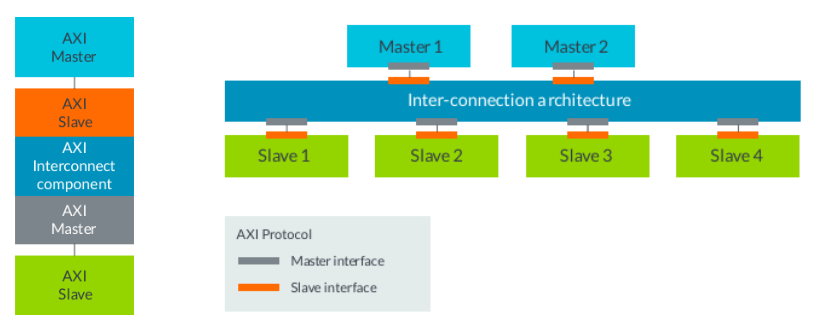
\includegraphics[width=1\linewidth]{chapter02/img/axi1.png}
    \caption{Sơ đồ AXI (AMBA)}
    \label{fig:placeholder}
\end{figure}

\subsection{Cơ sở lý thuyết và Cơ chế hoạt động của AXI4}
Giao thức AXI4 hoạt động dựa trên cơ chế ánh xạ bộ nhớ (Memory-Mapped I/O). Trong kiến trúc này, vi xử lý trung tâm không giao tiếp với các thiết bị ngoại vi thông qua các lệnh I/O đặc biệt, mà coi toàn bộ các khối phần cứng (Slave) như những dải địa chỉ bộ nhớ (Memory Addresses) liền kề \cite{arm_axi4_intro}.

\begin{figure}[!h]
    \centering
    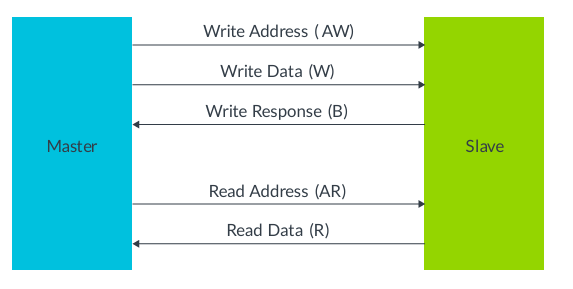
\includegraphics[width=1\linewidth]{chapter02/img/axi2.png}
    \caption{Các kênh giao tiếp (AMBA)}
    \label{fig:placeholder}
\end{figure}

Để đảm bảo hiệu suất truyền tải cao và hỗ trợ thực thi không theo thứ tự (Out-of-order execution), kiến trúc AXI4 phân tách các luồng dữ liệu thành 5 kênh (channels) độc lập, hoạt động song song và truyền theo một chiều duy nhất:
\begin{enumerate}
    \item \textbf{Kênh Địa chỉ Đọc (Read Address Channel - AR):} Truyền tải địa chỉ bắt đầu và các thông tin điều khiển cho quá trình đọc.
    \item \textbf{Kênh Dữ liệu Đọc (Read Data Channel - R):} Truyền dữ liệu từ Slave về Master, kèm theo cờ báo trạng thái đọc.
    \item \textbf{Kênh Địa chỉ Ghi (Write Address Channel - AW):} Truyền tải địa chỉ bắt đầu cho quá trình ghi dữ liệu.
    \item \textbf{Kênh Dữ liệu Ghi (Write Data Channel - W):} Truyền dữ liệu thực tế từ Master xuống Slave.
    \item \textbf{Kênh Phản hồi Ghi (Write Response Channel - B):} Slave phản hồi lại Master về trạng thái của toàn bộ giao dịch ghi (thành công hoặc có lỗi).
\end{enumerate}

\textbf{Cơ chế bắt tay:} 
Điểm cốt lõi làm nên độ tin cậy của AXI là cơ chế bắt tay hai chiều thông qua cặp tín hiệu \texttt{VALID} và \texttt{READY} có mặt trên tất cả 5 kênh. Master kéo tín hiệu \texttt{VALID} lên mức logic cao (1) để thông báo rằng dữ liệu hoặc địa chỉ trên bus đã hợp lệ. Ngược lại, Slave báo hiệu khả năng tiếp nhận bằng cách kéo tín hiệu \texttt{READY} lên cao. Một gói dữ liệu chỉ được coi là truyền thành công khi và chỉ khi cả \texttt{VALID} và \texttt{READY} đều ở mức 1 tại thời điểm sườn lên của xung nhịp (Clock Edge). Cơ chế này cho phép các khối phần cứng hoạt động ở các tần số xung nhịp khác nhau có thể đồng bộ hóa mà không gây ra hiện tượng mất mát dữ liệu hay thắt cổ chai (bottleneck).

\subsection{Phân loại các biến thể AXI trên nền tảng Xilinx}
Theo tài liệu \textit{Vitis Model Composer User Guide (UG1483)} của AMD/Xilinx \cite{ug1483}, giao thức AXI là tiêu chuẩn xương sống để đóng gói và kết nối các khối phần cứng. Tài liệu quy định quy trình ánh xạ (mapping) tự động các tín hiệu thuật toán cấp cao xuống ba biến thể AXI vật lý chính nhằm tối ưu hóa tài nguyên phần cứng và băng thông trên nền tảng FPGA:

\begin{itemize}
    \item \textbf{AXI4-Lite (Giao tiếp điều khiển vô hướng - Scalar):} 
    Theo UG1483, AXI4-Lite được sử dụng mặc định để ánh xạ các cổng tín hiệu đầu vào/đầu ra dạng vô hướng và các tín hiệu điều khiển (Control signals). Giao diện này tạo ra một bảng địa chỉ thanh ghi (Memory-Mapped Registers). Với đặc tính chỉ hỗ trợ truyền một đơn vị dữ liệu trong mỗi giao dịch (Single beat) và thiết kế logic cực kỳ nhỏ gọn, AXI4-Lite phù hợp để vi xử lý đọc/ghi trực tiếp vào các thanh ghi tĩnh của mạch gia tốc. Các thao tác điển hình bao gồm: ghi bit 1 để khởi động mạch (Start), đọc bit cờ báo hoàn thành (Done/Idle), hoặc nạp các tham số siêu tham số (Hyper-parameters) cho thuật toán.

    \item \textbf{AXI4 Memory-Mapped (AXI4-Full - Truy xuất khối tốc độ cao):} 
    Biến thể này được ứng dụng khi mô hình thiết kế cần giao tiếp với bộ nhớ đệm dùng chung dung lượng lớn như DDR RAM hoặc Block RAM (BRAM). Sức mạnh của AXI4-Full nằm ở khả năng truyền dữ liệu theo lô (Burst Transfer). CPU hoặc bộ điều khiển DMA (Direct Memory Access) chỉ cần cung cấp địa chỉ bắt đầu một lần duy nhất, sau đó có thể vận chuyển hàng ngàn byte dữ liệu (ví dụ: các bản đồ đặc trưng - Feature Maps của mạng CNN hoặc trọng số Weight) trong một chu kỳ thiết lập. Tính năng này giải quyết triệt để vấn đề "Bức tường bộ nhớ" (Memory Wall) trong các thiết kế gia tốc phần cứng AI.

    \item \textbf{AXI4-Stream (Dữ liệu luồng hướng sự kiện):} 
    Tài liệu chỉ định AXI4-Stream cho các luồng dữ liệu mảng (Array) tốc độ cực cao, phổ biến trong Xử lý tín hiệu số (DSP) và Xử lý ảnh (Vision AI). Khác biệt hoàn toàn với hai biến thể trên, AXI4-Stream truyền dữ liệu mà không cần địa chỉ bộ nhớ (Address-less). Nó hoạt động như một đường ống nước (Pipeline) kết nối trực tiếp đầu ra của khối này vào đầu vào của khối kia. Giao thức này chỉ sử dụng cơ chế bắt tay \texttt{TVALID} và \texttt{TREADY} để đẩy thông lượng (Throughput) lên mức tối đa mà không bị giới hạn bởi chu kỳ giải mã địa chỉ.
\end{itemize}

\subsection{Tích hợp hệ thống}

\textbf{Quy trình đóng gói phần cứng (IP Packaging):}
Một điểm nhấn quan trọng trong hệ sinh thái thiết kế của Xilinx (UG1483) là khả năng tự động hóa việc đóng gói. Khi thiết kế lõi thuật toán bằng ngôn ngữ mô tả phần cứng (Verilog/SystemVerilog), công cụ IP Packager không chỉ tổng hợp mạch logic lõi mà còn tự động sinh ra lớp bọc (wrapper) chứa các giao diện AXI chuẩn mực. Đồng thời, hệ thống cũng tự động khởi tạo bộ thư viện trình điều khiển phần mềm (C/C++ Driver API / BSP). Điều này cho phép hệ điều hành hoặc mã Bare-metal dễ dàng tương tác với khối phần cứng thông qua các hàm truy xuất thanh ghi tiêu chuẩn trong môi trường Vitis thống nhất.

\textbf{Ứng dụng chuẩn AXI vào Kiến trúc Gia tốc Mạng nơ-ron:}
Dựa trên nền tảng lý thuyết của giao thức AXI, kiến trúc của đồ án được định hình xoay quanh việc triển khai hệ thống nhận diện vật thể ứng dụng mô hình CNN lượng tử hóa (INT8) trên SoC Zynq UltraScale+ (Kit phát triển Kria KV260). Hệ thống là sự kết hợp đồng bộ giữa phần mềm chạy trên tập lệnh RISC-V (lõi mềm CV32E40P) và phần cứng gia tốc logic (CNN Accelerator). Giao thức AXI đóng vai trò cốt lõi trong việc định tuyến toàn bộ luồng điều khiển và luồng dữ liệu của thiết kế:

\begin{itemize}
    \item \textbf{Luồng Điều khiển (Control Flow) với AXI4-Lite:} Khối gia tốc phần cứng được tích hợp cổng giao tiếp Slave AXI4-Lite, được ánh xạ vào một dải địa chỉ cơ sở tĩnh trên không gian bộ nhớ của hệ thống (Memory-mapped). Vi xử lý trung tâm sử dụng đường truyền này để can thiệp trực tiếp vào máy trạng thái (FSM) của khối CNN. Cụ thể, các lệnh ghi/đọc được sử dụng để kích hoạt cờ vận hành (Start), hoặc kiểm tra trạng thái hoạt động (Status/Done). Để tối ưu hóa thời gian tính toán song song, hệ thống được thiết kế kết hợp phát tín hiệu ngắt cứng (IRQ) qua bộ điều khiển ngắt, giải phóng CPU khỏi việc phải liên tục chờ đợi vòng lặp (Polling).
    
    \item \textbf{Luồng Dữ liệu (Data Flow) với Kiến trúc Bộ nhớ dùng chung (Shared Memory):} Để giải quyết bài toán thắt cổ chai dữ liệu khi cả lõi RISC-V và lõi gia tốc CNN cùng cần truy xuất thông tin, hệ thống sử dụng một khối Block RAM (BRAM) cấu hình cổng kép (True Dual-Port BRAM) làm vùng nhớ dùng chung. Giao diện AXI4 kết nối vùng vi xử lý Host (nhân Cortex-A) và lõi RISC-V vào hệ thống BRAM này. Ban đầu, vi xử lý Host đóng vai trò quản lý tài nguyên, thực hiện nạp firmware cho RISC-V và đưa dữ liệu ảnh đầu vào (Inference Data) xuống BRAM thông qua bus AXI. Sau khi giải phóng tín hiệu Reset, lõi RISC-V sẽ trực tiếp nạp lệnh từ BRAM và đóng vai trò điều khiển độc lập để chỉ đạo khối CNN tính toán.
\end{itemize}

Việc tuân thủ chặt chẽ tiêu chuẩn giao tiếp AMBA AXI trong thiết kế này không chỉ đảm bảo hệ thống vận hành ổn định trên nền tảng FPGA Kria KV260, mà còn mang ý nghĩa lớn về mặt kiến trúc. Nền tảng Zynq hiện tại đóng vai trò là môi trường ASIC Prototyping. Khi định hướng đưa hệ thống vi mạch Edge AI này vào sản xuất thực tế (Tape-out), toàn bộ lõi RISC-V và bộ gia tốc CNN chuẩn AXI có thể được tái sử dụng trực tiếp trên đế Silicon (ASIC) mà không cần phải tái cấu trúc giao thức giao tiếp, khẳng định tính chuyên nghiệp và định hướng công nghiệp của đồ án.
%=================================================
%
%=================================================
\newpage
\section{tổng quan về trí tuệ nhân tạo (ai)}
\label{sec:ai_overview}

\subsection{Các Mô hình AI (AI Models)}
Trong lĩnh vực thị giác máy tính và hệ thống nhúng, các mô hình AI thường được phân loại dựa trên chức năng và kiến trúc. Việc lựa chọn mô hình phù hợp là yếu tố quyết định đến hiệu năng của hệ thống Edge AI.

\subsubsection{Mô hình Phân loại (Classification)}
Đây là dạng mô hình cơ bản nhất, nhiệm vụ là gán nhãn cho một hình ảnh đầu vào. Ví dụ: xác định xem trong ảnh có người hay không. Các kiến trúc tiêu biểu bao gồm MobileNet, SqueezeNet, và ResNet. Đối với các thiết bị biên, MobileNet thường được ưu tiên nhờ kiến trúc Depthwise Separable Convolution giúp giảm đáng kể khối lượng tính toán.

\subsubsection{Mô hình Phát hiện đối tượng (Object Detection)}
Phức tạp hơn phân loại, mô hình này không chỉ xác định đối tượng là gì mà còn định vị vị trí của nó thông qua các khung bao (Bounding Box). Các đại diện nổi bật gồm dòng YOLO (You Only Look Once) và SSD (Single Shot MultiBox Detector). Tuy nhiên, việc triển khai Object Detection trên soft-core RISC-V đòi hỏi tài nguyên tính toán rất lớn.

\subsubsection{Mô hình Phân đoạn (Segmentation)}
Phân loại từng pixel trong ảnh, giúp tách nền và đối tượng một cách chi tiết. Dạng mô hình này (ví dụ: U-Net) thường yêu cầu bộ nhớ lớn để lưu trữ các bản đồ đặc trưng (feature maps) độ phân giải cao, do đó ít được ưu tiên trên các hệ thống FPGA tài nguyên thấp nếu không có bộ tăng tốc phần cứng chuyên dụng.

\subsection{Training và Inference}
Để triển khai AI trên phần cứng, cần phân biệt rõ hai giai đoạn:
\begin{itemize}
    \item \textbf{Huấn luyện (Training):} Quá trình tìm ra bộ trọng số (weights) tối ưu cho mô hình thông qua việc học từ dữ liệu lớn. Quá trình này yêu cầu tính toán dấu phẩy động (Float32/Float16) và thường thực hiện trên Server hoặc GPU mạnh.
    \item \textbf{Suy luận (Inference):} Quá trình sử dụng mô hình đã huấn luyện để đưa ra dự đoán trên dữ liệu mới. Tại thiết bị biên (Edge), suy luận yêu cầu độ trễ thấp và thường sử dụng kỹ thuật lượng tử hóa để chạy trên phần cứng số nguyên (Integer hardware) như RISC-V soft-core.
\end{itemize}

\subsection{Phân loại AI và Mối liên hệ với Deep Learning}
Trí tuệ nhân tạo là một thuật ngữ rộng, bao hàm nhiều cấp độ:
\begin{itemize}
    \item \textbf{AI hẹp (Narrow AI):} Các hệ thống được thiết kế cho một tác vụ cụ thể (như nhận dạng ảnh trong đề tài này).
    \item \textbf{Học máy (Machine Learning - ML):} Tập con của AI, nơi máy tính học từ dữ liệu thay vì được lập trình quy tắc cứng.
    \item \textbf{Học sâu (Deep Learning - DL):} Tập con của ML, sử dụng các mạng nơ-ron nhiều lớp để trích xuất đặc trưng tự động.
\end{itemize}
\textit{Chi tiết về cấu trúc và nguyên lý hoạt động của Mạng nơ-ron nhân tạo (ANN) và Học sâu sẽ được trình bày chuyên sâu tại Mục \ref{sec:neural_network}.}

\subsection{Edge AI}

\subsubsection{Khái niệm}
Edge AI là sự kết hợp giữa thuật toán AI và tính toán biên (Edge Computing), cho phép xử lý dữ liệu cục bộ ngay trên thiết bị phần cứng mà không cần gửi dữ liệu về trung tâm dữ liệu (Cloud).

\subsubsection{Ưu điểm so với Cloud AI}
\begin{itemize}
    \item \textbf{Độ trễ thấp (Low Latency):} Phản hồi tức thời, phù hợp cho các ứng dụng thời gian thực (ví dụ: xe tự lái, robot).
    \item \textbf{Bảo mật và Quyền riêng tư:} Dữ liệu hình ảnh nhạy cảm không rời khỏi thiết bị, giảm nguy cơ bị tấn công đường truyền.
    \item \textbf{Tiết kiệm băng thông:} Không cần truyền tải luồng video liên tục lên máy chủ, giảm tải cho hạ tầng mạng.
    \item \textbf{Độ tin cậy:} Hệ thống vẫn hoạt động bình thường ngay cả khi mất kết nối Internet.
\end{itemize}

\subsubsection{Các Framework phổ biến cho Edge AI}
\begin{itemize}
    \item \textbf{TensorFlow Lite (TFLite):} Phiên bản rút gọn của TensorFlow, tối ưu cho thiết bị di động và nhúng. TFLite hỗ trợ chuyển đổi mô hình sang định dạng FlatBuffer nhẹ và cung cấp các toán tử tối ưu cho vi xử lý ARM và RISC-V.
    \item \textbf{Vitis AI:} Nền tảng phát triển của AMD-Xilinx, chuyên dụng để tối ưu hóa mô hình AI chạy trên các kiến trúc DPU (Deep Learning Processor Unit) của FPGA Xilinx.
    \item \textbf{ONNX Runtime:} ONNX (Open Neural Network Exchange) là định dạng trung gian giúp chuyển đổi mô hình giữa các framework (PyTorch sang TensorFlow). ONNX Runtime cho phép chạy suy luận hiệu năng cao trên nhiều nền tảng phần cứng khác nhau.
\end{itemize}

%=================================================
%=================================================
\section{Mạng Nơ-ron Nhân tạo (Artificial Neural Networks)}
\label{sec:neural_network}

Mạng nơ-ron nhân tạo (ANN) là nền tảng của Deep Learning, 
lấy cảm hứng từ cơ chế truyền dẫn tín hiệu điện hóa giữa các nơ-ron 
trong bộ não sinh học. Trước khi đi sâu vào kiến trúc CNN được sử dụng trong đề tài, 
cần xem xét tổng quan các kiến trúc mạng nơ-ron phổ biến để thấy rõ sự phù hợp 
của từng loại đối với các tác vụ cụ thể.\cite{CNN}

\subsection{Các kiến trúc Mạng Nơ-ron phổ biến}

\subsubsection{Mạng Nơ-ron Truyền thẳng (Feedforward Neural Network - MLP)}
Đây là dạng đơn giản nhất của ANN, còn được gọi là Multi-Layer Perceptron (MLP). Trong kiến trúc này, thông tin di chuyển theo một chiều từ lớp đầu vào (Input), qua các lớp ẩn (Hidden layers) đến lớp đầu ra (Output) mà không có chu trình quay lại.
\begin{itemize}
    \item \textbf{Đặc điểm:} Các nơ-ron ở lớp trước kết nối đầy đủ (fully connected) với nơ-ron lớp sau.
    \item \textbf{Hạn chế với hình ảnh:} Khi xử lý ảnh, MLP làm mất thông tin không gian (spatial structure) do phải duỗi phẳng ảnh thành vector 1 chiều. Ngoài ra, số lượng tham số bùng nổ quá nhanh dẫn đến quá tải bộ nhớ và hiện tượng quá khớp (overfitting).
\end{itemize}

\subsubsection{Các kiến trúc khác}
Ngoài MLP, lĩnh vực mạng nơ-ron còn có Mạng nơ-ron Hồi quy (RNN, với các biến thể LSTM/GRU) chuyên cho dữ liệu chuỗi thời gian, và Vision Transformers (ViT) áp dụng cơ chế Self-Attention. Tuy nhiên, RNN không hiệu quả trong việc trích xuất đặc trưng không gian 2D và khó song song hóa, còn ViT có độ phức tạp $O(N^2)$ tiêu tốn tài nguyên rất lớn -- cả hai đều không phù hợp với ràng buộc của một soft-core RISC-V trên FPGA tài nguyên hạn chế. Do đó, đồ án lựa chọn Mạng nơ-ron Tích chập (CNN) làm kiến trúc chính, sẽ được trình bày tại mục~\ref{sec:cnn}.

\subsection{Mạng Nơ-ron Tích chập (CNN)}
\label{sec:cnn}
Dựa trên phân tích trên, CNN là kiến trúc cân bằng nhất giữa hiệu năng và chi phí tính toán cho các thiết bị biên. CNN là kiến trúc mạng chuyên biệt cho dữ liệu dạng lưới (grid-like topology) như hình ảnh. Một mạng CNN điển hình bao gồm ba loại lớp chính:

\subsubsection{Lớp Tích chập (Convolutional Layer)}

Đây là lớp quan trọng nhất, thực hiện trích xuất đặc trưng cục bộ và bảo toàn tính chất không gian của ảnh. Phép tính tích chập là việc trượt một cửa sổ nhỏ (Kernel/Filter) trên toàn bộ ảnh đầu vào và thực hiện phép nhân chập.
Về mặt toán học, giá trị đầu ra $Y$ tại vị trí $(i, j)$ được tính như sau:
\begin{equation}
Y[i, j] = \sum_{m} \sum_{n} X[i+m, j+n] \cdot K[m, n] + b
\end{equation}
Trong đó: $X$ là ma trận đầu vào, $K$ là ma trận Kernel, và $b$ là bias. Trên các vi xử lý RISC-V hỗ trợ DSP (như Pulpino), phép toán này có thể được tăng tốc bằng các lệnh SIMD (Single Instruction Multiple Data), cho phép thực hiện 4 phép nhân 8-bit trong một chu kỳ xung nhịp.

\subsubsection{Hàm kích hoạt (Activation Function)}
Hàm kích hoạt giúp đưa tính phi tuyến vào mô hình, cho phép mạng học được các đặc trưng phức tạp. Hàm phổ biến nhất trong CNN là \textbf{ReLU (Rectified Linear Unit)}:
\begin{equation}
f(x) = \max(0, x)
\end{equation}
ReLU có ưu điểm lớn về mặt tính toán trên phần cứng nhúng vì chỉ cần một lệnh so sánh đơn giản (nếu $x < 0$ thì gán bằng 0), không tốn kém tài nguyên như hàm Sigmoid hay Tanh (vốn yêu cầu tính toán số mũ thực rất nặng nề cho soft-core).

\subsubsection{Lớp Gộp (Pooling Layer)}
Dùng để giảm kích thước không gian của bản đồ đặc trưng (down-sampling), giúp giảm số lượng tham số và tính toán, đồng thời giúp mô hình bất biến với các dịch chuyển nhỏ (Translation Invariance) của đối tượng. Hai kỹ thuật phổ biến là Max Pooling (lấy giá trị lớn nhất) và Average Pooling (lấy giá trị trung bình).

\subsection{Kỹ thuật Lượng tử hóa (Quantization)}
Lượng tử hóa là kỹ thuật cốt lõi để triển khai AI trên các vi xử lý RISC-V soft-core không có bộ xử lý dấu phẩy động (FPU) mạnh mẽ.

\subsubsection{Khái niệm}
Kỹ thuật này chuyển đổi các trọng số (weights) và giá trị kích hoạt (activations) từ dạng số thực 32-bit (Float32) sang số nguyên 8-bit (Int8). Công thức chuyển đổi tổng quát:
\begin{equation}
r = S \times (q - Z)
\end{equation}
Trong đó: $r$ là giá trị thực, $q$ là giá trị lượng tử hóa (int8), $S$ là tỉ lệ (Scale factor), và $Z$ là điểm không (Zero-point).

\subsubsection{Lợi ích trên FPGA/RISC-V}
\begin{itemize}
    \item \textbf{Giảm bộ nhớ:} Kích thước mô hình giảm 4 lần (từ 32-bit xuống 8-bit), giúp mô hình vừa vặn với bộ nhớ on-chip (BRAM/TCM) hạn hẹp của FPGA, giảm độ trễ truy cập bộ nhớ ngoài (DDR).
    \item \textbf{Tăng tốc độ:} Các phép tính số học trên số nguyên (Integer Arithmetic) nhanh hơn và tiêu thụ ít năng lượng hơn nhiều so với số thực. Các nhân RISC-V như RI5CY hỗ trợ thực hiện 4 phép nhân cộng Int8 trong một chu kỳ máy.
\end{itemize}

\subsection{Các kỹ thuật tối ưu hóa khác}

\subsubsection{Kỹ thuật Cắt tỉa }
Pruning loại bỏ các kết nối (trọng số) có giá trị gần bằng 0 hoặc ít ảnh hưởng đến kết quả đầu ra. Kỹ thuật này biến ma trận trọng số dày đặc (Dense) thành ma trận thưa (Sparse), giúp giảm đáng kể khối lượng tính toán và bộ nhớ lưu trữ mà không làm giảm nhiều độ chính xác.

\subsubsection{Kỹ thuật im2col (Image-to-Column)}

Để tối ưu hóa phép tính tích chập trên phần cứng, kỹ thuật \textit{im2col} thường được sử dụng. Nó biến đổi ma trận ảnh đầu vào thành các cột, chuyển bài toán tích chập phức tạp (Convolution) thành bài toán nhân ma trận (GEMM - General Matrix Multiply). GEMM là phép toán đã được tối ưu hóa rất tốt trên các thư viện tính toán (như BLAS) và tận dụng triệt để khả năng xử lý song song.

Trong đồ án này, bộ tăng tốc Conv-CNN v2.0 không sử dụng \textit{im2col} vì áp dụng kiến trúc \textit{streaming dataflow} với line buffer + window register: dữ liệu được trượt qua window $3 \times 3$ và đưa vào trực tiếp 9 PE MAC, tránh chi phí biến đổi và sao chép bộ nhớ của \textit{im2col}.
